\documentclass{article}
\usepackage[utf8]{inputenc}
\usepackage[a4paper, portrait, margin=1in]{geometry}
\usepackage{tabularx}
\usepackage{graphicx}
\usepackage{amsmath}
\usepackage{hyperref}
\hypersetup{
    colorlinks=true,
    linkcolor=blue,
    filecolor=magenta,      
    urlcolor=cyan,
}


\title{OOAD \& Software Engineering (UE18CS353) \\
    Unit 5}
\author{Aronya Baksy}
\date{April 2021}

\begin{document}
\maketitle
\section{Ethics in SE}
\begin{itemize}
    \item Professional ethics: guiding principles for ideal behaviour and actions in a professional environment
    
    \item SE Ethics becomes important when design/implementation/maintenance decisions taken during the development affect real people. 
    
    \item All decisions taken during software engineering must be guided by technical as well as ethical considerations. Software design must incorporate ethics.
    
    \item Code of Ethics is a generic term used for a document that describes the interaction between ethics and technology. CoE ensures that this interaction is structured, and may/may not carry legal weight.
\end{itemize}
\subsection{Code of Ethics}
\begin{itemize}
    \item Guiding principles in understanding boundaries and guides the behaviour of  free agents in taking decisions
    
    \item Integrity, objectivity, competence, confidentiality, behaviour wrt. resource usage, respect for Intellectual Property
\end{itemize}

\subsection{Code of Conduct}
\begin{itemize}
    \item Day-to-day behaviour of employees at the workplace. 
    
    \item Equality, fairness, empathy, respect, compliance with laws/standards/guidelines, portraying realistic competence level. 
\end{itemize}

\subsection{Eight Principles}
\begin{itemize}
    \item Act with \textbf{pulbic} interest in mind
    
    \item Act in a manner that is in the best interest of \textbf{client and employer} while keeping the above in mind
    
    \item Build \textbf{products} that meet the highest professional standards of quality.
    
    \item Maintain integrity and independence in professional \textbf{judgement}
    
    \item Promote an ethical approach to \textbf{management} of Software development and maintenance
    
    \item Advance integrity and reputation of the \textbf{profession}. 
    
    \item Be fair to and support your \textbf{colleagues}
    
    \item \textbf{Self}: engage in lifelong learning, promote ethical approach to the professsion of software engineering. 
\end{itemize}

\subsection{Hacking}
\begin{itemize}
    \item Hackers solve problems in non-standard methods (e.g. exploiting weaknesses of systems). Motivated more by novelty/challenges as against traditional rewards like \$\$\$ and power.
    
    \item Hacking involves poking around with multiple solutions to see which one works best. May lead to traceability issues due to the lack of documentation associated with hacking.
    
    \item Engineers, by contrast, take solutions to existing problems and seek to improve their non-functional attributes (aesthetics, reliability, performance benchmarks) through technical solutions, within a budget and time constraint. 
    
    \item Engineering involves crafting a solution understanding why and the considering the best practices.
    
    \item Computer hackers are classified as 
    \begin{itemize}
        \item \textbf{White-Hat}: improve organization security by finding vulnerabilites, design solutions to patch them up
        
        \item \textbf{Black-Hat}: look for exploits in organization security that can be used for gathering data for purposes such as corporate espionage, nation-state hacking etc.
    \end{itemize}
\end{itemize}

\section{Global Software Engineering}
\begin{itemize}
    \item Traditional approach: co-located teams working on inter-related goals. 
    
    \item Global Development Team: Use virtual teams to develop software, linked by communication technologies and working remotely. 
    
    \item Global distance = geographical distance + linguistic distance + temporal (time-zone) distance + cultural distance
    
    \item Software teams can be organized as \textbf{co-located}, \textbf{multi-site} or \textbf{global} (multi-site teams organized across $>1$ country)
    
    \item Advantages of global development:
    \begin{itemize}
        \item Increase productivity hours, leads to faster delivery
        
        \item Larger pool of global developers, keep teams closer to clients 
        
        \item Diverse stakeholders with diverse knowledge and experience. 
    \end{itemize}
    \item Communication, Teaming, Collaboration and Project management practices and processes if put in plan can mitigate the challenges of Global development. 
\end{itemize}
\subsection{Challenges and Solutions in Global SE}
\begin{itemize}
    \item \textbf{Communication}: involve less informal communication, build trust through team-building activites
    
    \item \textbf{Coordination}: ensure shared sense of urgency, and task awareness
    
    \item \textbf{Control}: use accurate tools for tracking issues and progress, maintain uniform process across locations
    
    \item \textbf{Culture}: Build awareness about social backgrounds, attitudes, cultural distances
\end{itemize}

\section{ITSM and ITIL}
\subsection{IT Service Management (ITSM)}
\begin{itemize}
    \item ITSM processes manage deployment of software products in real-world environments. 
    
    \item ITSM is about how an IT organization manages IT services for customers and provides a stable IT environment that supports the business. 
    
    \item THe objectives of ITSM are:
    \begin{itemize}
        \item Improved availability, security, reliability of IT infrastructure
        
        \item Increased flexibility, productivity, scaling
        
        \item Predictable support and reduction in costs
    \end{itemize}
\end{itemize}

\subsection{ITSM Processes}
\subsubsection{Availability Management}
\begin{itemize}
    \item Manage expectations of agreed-upon level of functioning of services in a cost-effective and efficient manner
    
    \item The 7 Rs (Reliability, Redundancy, Repairability, Recoverability, Responsiveness, Robustness, Reputation)
\end{itemize}

\subsubsection{Performance/Tuning}
\begin{itemize}
    \item Performance optimization for increased throughput, minimized response time even in the face of dynamic workloads
    
    \item For networks, storage devices, servers, databases
\end{itemize}

\subsubsection{Acceptance}
\begin{itemize}
    \item Methodology for consistently deploying software to a production environment regardless of environment etc.
    
    \item Maintain integrity of application post deployment
\end{itemize}

\subsubsection{Change Management}
\begin{itemize}
    \item Changes made to IT environment for improvement of performance/reliability etc., or for fixing existing issues in the environment
    
    \item Involves change control (request, prioritize, approval) and co-ordination (collaboration, schedule, communicate and implement)
\end{itemize}

\subsubsection{Problem Management}
\begin{itemize}
    \item Log, track, analyze and resolve problems raised in the IT environment.
    
    \item When client initiates a call, the problem is analyzed and added for tracking and logging
\end{itemize}

\subsubsection{Storage and Network Management}
\begin{itemize}
    \item Increase performance, reliability, utilization of storage and network devices.
\end{itemize}

\subsubsection{Configuration Management}
\begin{itemize}
    \item Document relationships between different versions of software and hardware components in the IT infrastructure
\end{itemize}

\subsubsection{Capacity Management}
\begin{itemize}
    \item Predict and provision resources as needed (when, what type, how much) needed based on predicted workload of the system
\end{itemize}

\subsubsection{Strategic Security Management}
\begin{itemize}
    \item Safeguard the security, integrity and confidentiality of the IT environment against unauthorized access, modification and deletion
    
    \item Achieved through security testing, security reviews and security incidents.
\end{itemize}

\subsubsection{Business Continuity Process}
\begin{itemize}
    \item Managing normal continuous operation of the environment in the event of disasters that affect the environment.
    
    \item Business continuity involves risk identification (in terms of disasters), risk mitigation plans (to minimize the risk impact) and risk recovery plans to get the environment back to operation soon after a disaster occurs.
\end{itemize}

\subsection{IT Infrastructure Library (ITIL)}
\begin{itemize}
    \item A framework or a set of ITSM best practices that focus on aligning business goals with IT development goals
    
    \item These best practices are not organization or technology specific, but are generic, used for establishing integration with the business strategy, generating value and maintaining basic competency.
    
    \item ITIL is a public-domain framework. Started in the UK in the 1980s, with around 40 volumes, current ITIL v4 (2019) is around 60 volumes long.
\end{itemize}

\subsubsection{ITIL v3 life cycle}
\begin{itemize}
    \item \textbf{Service Strategy}: Understand business objectives and customer needs, provide strategic guidance for investments in services. Includes service value definition, business-case development, service assets, market analysis, and service provider types
    
    \item \textbf{Service Design}: Turn the strategy into a detailed plan that outlines the delivery of the service and business objectives
    
    \item \textbf{Service Transition}: Develop capabilities for introducing new services in an existing environment, relates to the "delivery" of services. 
    
    \item \textbf{Service Operation}: Manages services in supported environments,  provide best practice for achieving the delivery of agreed service level both to end-users and the customers. Includes Ops management, Service management, Service desks etc.
    
    \item \textbf{Service Improvement}: Incremental and large-scale improvements in delivered services. 
\end{itemize}

\subsubsection{ITIL v4}
\begin{itemize}
    \item Consists of 34 management practices subdivided into:
   
    \item \textbf{General management practices} including architecture management, measurement and reporting, risk management and project management 
    
    \item \textbf{Technical management practices} which include Infrastructure and platform management and software development and management  
    
    \item \textbf{Service management practices} like Availability management, Capacity management and performance management, Incident management etc.
\end{itemize}
\section{DevOps}
\begin{itemize}
    \item DevOps is the combination of philosophies, practices and tools that increase the ability of an organization to deliver (i.e. deploy and support) effective software applications at high velocity.
    
    \item It is the result of Software Development and IT Operations working in synchronization
    
    \item The software devleopment team's activites are controlled by the SDLC, while the IT Operations team takes care of utilization of IT infrasturcture owned by the developing organization.
    
    \item DevOps aims to remove repetitive manual processes; these are automated as much as possible. 
    
    \item DevOps follows the Agile principle of prioritizing individuals and interactions, over processes and tools. 
    
    \item DevOps leads to faster delivery and deployment (maybe several times a day using CI/CD pipelines)
    
    \item The four common themes or pillars that are required for implementation of DevOps in an organization are:
    \begin{itemize}
        \item Collaboration
        
        \item Affinity
        
        \item Tools
        
        \item Scaling
    \end{itemize}
\end{itemize}

\subsection{Pillars of DevOps}
\subsubsection{Collaboration}
\begin{itemize}
    \item Working towards a common objective with the interaction and support of multiple teams and individuals 
    
    \item Collaboration is based on: 
    \begin{itemize}
        \item Communication
        
        \item Equal participation
        
        \item Theory of Mind, which is the ability to recognize one's perspective and understanding that others have distinct perspectives based on their own context
    \end{itemize}
    
    \item Collaboration necessitates relationships based on trust and empathy (empathy for different socio-cultural, economic and professional backgrounds, as well as different cognitive styles and professional goals/needs)
    
    \item Less established hierarchies, more supporting opportunities (mentorships, sponsorships)
\end{itemize}

\subsubsection{Affinity}
\begin{itemize}
    \item The measure of strength of a relationship between individuals, teams, business units or even companies. 
    
    \item Relationships are strengthened by navigating differing goals or metrics while keeping in mind shared goals, as well as creating empathy and learning between different groups.
    
    \item Affinity is \textbf{measured} using:
    \begin{itemize}
        \item Shared time
        
        \item Reciprocity of stories and support
        
        \item Intensity of relationship
    \end{itemize}
    
    \item Affinity is \textbf{built} using:
    \begin{itemize}
        \item Shared values
        
        \item Team cohesion
        
        \item Strong and consistent team culture
    \end{itemize}
\end{itemize}

\subsubsection{Tools}
\begin{itemize}
    \item Tools drive change based on current culture and direction. They are the common language using which different teams communicate
    
    \item Usability of tools drives team culture, a tool must be usable by all members of a team in order to build cohesion and trust in the team. 
    
    \item Examples of tools used in DevOps are unit testing tools, build tools, monitoring tools, tracking tools for issues etc.
\end{itemize}

\subsubsection{Scaling}
\begin{itemize}
    \item Application of DevOps principles and pillars as organizations change in size and structure 
    
    \item Involves technical and cultural considerations of operating at different scales
    
    \item Scaling could be for Organization, infrastructure, teams (hiring, retention, outsourcing), Complexity, Workload

\end{itemize}

\subsection{DevOps Pipeline}
\subsubsection{Version Control}
\begin{itemize}
    \item Record changes to files stored within a repository that is shared by multiple developers
    
    \item Changes can be saved by developers using commit operations. Changes may be made by an individual or group of developers.
    
    \item Richer collaboration is provided by the ability to compare changes, merge changes and restore past versions of the repository. 
\end{itemize}
\subsubsection{Continuous Integration (CI)}
\begin{itemize}
    \item Merging branches of the repository owned by individual developers with the master branch as frequently as possible (multiple times a day)
    
    \item Multiple developers can checkout their own branch from master, make changes on their own branch, and merge their branches with the master concurrently. 
    
    \item Merging of branches happens multiple times a day. Merge conflicts, if any, can be handled and the merge takes place. Metadata about each revision is stored by the system. 
    
    \item CI is in contrast to big-bang integration which has a higher chance of leading to integration failures or merge conflicts, and hence causing build failure later on. 
    \item Benefits of CI:
    \begin{enumerate}
        \item Early error detection, reduced debugging effort and time
        
        \item Small and incremental integrations are easier to manage
        
        \item Increased visibility and communication
    \end{enumerate}
\end{itemize}

\subsubsection{Continuous Build}
\begin{itemize}
    \item Building an executable application from the input code files. 
    
    \item Involves static analysis (linting, data-flow or control-flow analysis), followed by actual build and sanity testing
    
    \item \textbf{Sanity testing} checks that the build was successful, includes all dependencies and is in a runnable state. 
\end{itemize}
\subsubsection{Continuous Delivery}
\begin{itemize}
    \item Frequent deployment of code to a production or test environment. 
    
    \item Supports quick releases in a sustainable manner. 
    
    \item CD can be triggered automatically by a trigger at the end of the build process.
    
    \item Supports faster time to market, and deployment on demand. 
    
    \item Tools that support CD: Jenkins, CircleCI, GitLab, AWS CodeDeploy
\end{itemize}

\subsubsection{Continuous Testing}
\begin{itemize}
    \item Executing automated tests frequently as part of the DevOps pipeline allows the code to be in a deployable state most of the time, while detecting bugs as early as possible.
    
    \item Tests are designed to execute with minimal wait time, and provide instant feedback and bug discovery/prevention. 
    
    \item Tests involve static code analysis, validation of both functional and non-functional requirements
    
    \item Tests can be executed several times a day, using a trigger on the version control system (i.e. everytime someone pushes to the master branch, run the test suite)
\end{itemize}

\subsubsection{Continuous Deployment}
\begin{itemize}
    \item A software release process that uses delivery mechanisms for deploying the validated product, immediately and autonomously to a production environment.
    
    \item Validated and integrated components are batched together and are then deployed into customer environment
    
    \item Removes the need for moving code between 2 environments, checking if it works as expected (typically error prone and resource-heavy process). 
    
    \item Tools automate the entire deployment process, allows more focus on business golas than infrastructure overheads.
\end{itemize}
\begin{figure}[!h]
    \centering
    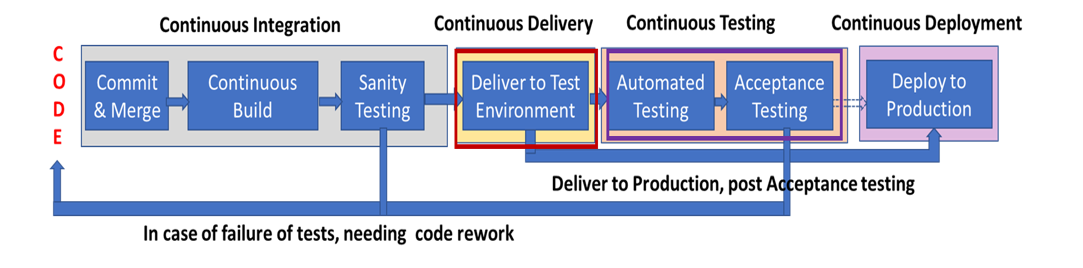
\includegraphics[scale=0.6]{p1.png}
    \caption{DevOps Pipeline}
    \label{fig:my_label}
\end{figure}
\begin{tabular}{|p{0.45\textwidth}|p{0.45\textwidth}|}
    \hline
    \textbf{DevOps} & \textbf{Agile}  \\
    \hline
    A culture and approach which looks to remove the silos of Development activities of building a product and the Operations activities of deployment, support and upkeep. & A process that supports changes, ensures more collaborations between developers and other stakeholders, reduces the planning overhead and delivers products or part of products periodically \\
    \hline
    Focus on constant test and delivery & Focus on constant change \\
    \hline
    Target is end-to-end business solutions and fast delivery & Target is efficient software development \\
    \hline 
    Operational and business readiness & Functional and non-functional readiness \\
    \hline
\end{tabular}
\end{document}